\documentclass[a4paper]{article}
\usepackage[dvipsnames]{xcolor}
\usepackage{amsfonts,amsmath,amstext,amssymb,caption,listings,mathtools,tikz}
\usepackage[dutch]{babel}
\usepackage{enumitem}
\captionsetup{width = 0.8\textwidth, font=small, textfont=it, labelfont=bf}
\addto\captionsdutch{%
  \def\lstlistingname{Programma}}
\addto\extrasdutch{
  \def\figureautorefname{Figuur}}



\usepackage[hidelinks,bookmarksopenlevel=3]{hyperref}
\usetikzlibrary{babel}
\setlength{\parindent}{0pt}
\setcounter{tocdepth}{3}
\newlength{\leftoflengthopdr}
%%%%%%%%%%
% Macrodefinities
%%%%%%%%%%
\makeatletter
\newcounter{opdracht}
\newcounter{deelopdracht}[opdracht]
\newcounter{niveaudummie}
\newcounter{dummie}

\definecolor{opdrachtkleur}{RGB}{204,0,0} %Initialiseer op RUG-rood
\definecolor{J1H2}{RGB}{204,102,0}
\definecolor{J2H6}{RGB}{132,133,255}
\definecolor{J3H5}{RGB}{175,0,175}

\lstset{
	keepspaces=true,
	frame=tBlR,
	rulesepcolor=\color{opdrachtkleur},
	numbers=left,
	tabsize=2,
	breaklines=true,
	breakatwhitespace=true,
	captionpos=b,
	postbreak={\mbox{$\cdots$}},
	prebreak={\mbox{$\cdots$}},
	mathescape=true,%
	}
	
\def\pijl{
	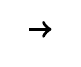
\begin{tikzpicture}[very thick,x=1em,y=1em,baseline={(0,-0.35em)}]
		\draw [->](-0.4,0) -- (0.4,0);
	\end{tikzpicture}
	}
\def\eindpijl{
	
\begin{tikzpicture}[very thick,x=1em,y=1em,baseline={(0,-0.3em)}]
		\draw[<-] (-0.25,0) -- (0.25,0) -- (0.25,0.3); 
	\end{tikzpicture}
	}
\def\vervolg{
	
\begin{tikzpicture}[very thick,x=1em,y=1em,baseline={(0,-0.3em)}]
		\draw[<-] (0.25,0) -- (-0.25,0) -- (-0.25,0.3); 
	\end{tikzpicture}%
	}
\def\dakje{
	
\begin{tikzpicture}[very thick,x=1em,y=1em,baseline={(0,0)}]
		\draw (-0.3,0.3) -- (0,0.7) -- (0.3,0.3);
	\end{tikzpicture}
	}
\def\dh{
	
\begin{tikzpicture}[very thick,x=1em,y=1em,baseline={(0,0)}]
		\filldraw (0,0) -- (0.3,0) -- (0.3,0.3) -- cycle;
	\end{tikzpicture}
	}
\def\sp{\bfseries\textvisiblespace}
\lstdefinestyle{basic}{%
	language=[Visual]Basic,%
	keywordstyle=\bfseries\underbar,%
	commentstyle=\itshape\small,%
	mathescape=true,%
	morekeywords={To,LpWhile,IfEnd,Step,Lbl,Locate,ClrText},%
	literate={->}{\pijl}1 {;}{\eindpijl}1{^}{\dakje}1{;;}{\dh}1%
	}
	
\lstdefinestyle{pascal}{%
	language=Pascal,
	keywordstyle=\bfseries\underbar,%
	commentstyle=\itshape\small,%
	mathescape=true,%
	deletekeywords=[1]{mod,false},%
	morekeywords={RETURN,EXPORT,LOCAL,FROM},
	morecomment=[l]{//},
}

\lstdefinelanguage{pseudo}
{
  % list of keywords
  morekeywords={invoer,uitvoer,voor,als,dan,anders,geef,print,zolang,zeg},
  sensitive=false, % keywords are not case-sensitive
  morecomment=[l]{//}, % l is for line comment
  morecomment=[s]{/*}{*/}, % s is for start and end delimiter
  morestring=[b]" % defines that strings are enclosed in double quotes
}

\def\lstsqrt#1{\raisebox{3pt}[\totalheight][0pt]{$\smash{\sqrt{#1}}$}}


\newif\if@beginopdracht

\colorlet{opdrachtkleur}{J1H2} %maak kleur
%\setcounter{opdracht}{0} Zie einde minipage
\def\nivset#1{\setcounter{niveaudummie}{#1}\Roman{niveaudummie}}
\def\opdracht{\@ifnextchar[{\opdrachtniv}{\opdrachtzonderniv}}
\def\opdrachtzonderniv#1{%
	\begin{tikzpicture}[baseline=(nodename.base)]
		 	\node[draw=opdrachtkleur,fill=opdrachtkleur,text=white] (nodename) {\bfseries #1};
		\end{tikzpicture}%
		}
\def\opdrachtniv[#1]{%
	\refstepcounter{opdracht}%
	\bigskip\bigskip%
	\makebox[0pt][r]{%
		\begin{tikzpicture}[baseline=(nodename.base)]
		 	\path[draw=opdrachtkleur] (-3em,-0.75em) rectangle (1em,0.75em);
		 	\node (nodename) [text=opdrachtkleur] at (-2em,0) {\bfseries\nivset{#1}};
		 	\path[draw=opdrachtkleur,fill=opdrachtkleur,text=white] (-1em,-0.75em) rectangle (1em,0.75em) (0,0) node {\bfseries P\theopdracht};
		\end{tikzpicture}%
		\hspace{\leftoflengthopdr}%
		}%
		\@beginopdrachttrue%
		\ignorespaces%
	}
\def\?{%
	\refstepcounter{deelopdracht}\if@beginopdracht\else{\hfill\\}\fi\makebox[1em][l]{\bfseries\thedeelopdracht}%
	\@beginopdrachtfalse%
	}
\def\refopdracht#1{%
		\@ifnextchar\bgroup%
		{\@deelopdrachtref{#1}}%
		{\opdracht{P\ref{#1}}}%
		}
\def\@deelopdrachtref#1#2{\opdracht{P\ref{#1}(\textbf{\ref{#2}})}}
\makeatother
\newcommand\ggd{\ensuremath{\operatorname{ggd}}}
\newcommand\kgv{\ensuremath{\operatorname{kgv}}}
\renewcommand\thedeelopdracht{\alph{deelopdracht}}

\let\labeloud\label
\def\label#1{\labeloud{#1}\ignorespaces}
%%%%%%%%%%
% Einde macrodefinities
%%%%%%%%%%
\author{Benny Aalders \and Vincent Velthuizen}
\title{\vspace*{-1.9in}Voorbeeld van een opdrachtenboek met {``Computational-Thinking-opdrachten''} aansluitend bij de methode {Getal \& Ruimte}}
\date{Versie: \today}

\begin{document}\maketitle
%\begin{abstract}
%	Het bestand dat voor u ligt betreft een in ontwikkeling zijnde versie. Wij (de auteurs) weten dat er nog ruimte is voor verbetering(en). Op bepaalde punten 
%\end{abstract}
In dit document staan voorbeeldopgaven die in een programmeerboek zouden kunnen staan dat wordt meegeleverd met een lesboek/een serie lesboeken. Bij wijze van voorbeeld hebben we voor de lesboekenserie Getal \& Ruimte  gekozen. 

Bij de opdrachten zijn niveaus aangegeven. Het meetniveau is ordinaal. Toewijzing van de niveaus is op dit moment enkel gebaseerd op onze eigen inschatting. De niveaus dienen louter om een vorm van structuur zichtbaar tijdens het ontwikkelingsproces. 

\paragraph{Niveaus I--II} Dit zijn opdrachten op instapniveau; i.e.: vertrouwd raken met de mogelijkheden en methodes. Dit zou voor vmbo het eindniveau  kunnen  zijn. 
Bij deze opdrachten is het programmeerniveau relatief laag of nul. Het draait hier meer om het gebruiken van de beschikbare technologie.

\paragraph{Niveau III} Dit zijn opdrachten waar programmeren een grotere rol speelt. Dit is voor havo/VWO bedoeld.  Bij het maken van deze opdrachten heeft de leerling alle basiskennis nodig over het bijbehorende hoofdstuk uit zijn lesboek. 

\paragraph{Niveau IV} Deze opdrachten gaan wat dieper in op de stof. Over het algemeen wordt hier getest wat een programma doet met ongebruikelijke invoer. 

Een voorbeeld: In \refopdracht {randvoorw}{negatief} wordt gevraagd wat er gebeurt wanneer je $\ggd(-2,4)$ met je programma probeert uit te rekenen. Een leerling moet dan nadenken over de precieze definitie van de \ggd\ en of $\ggd(-2,4)$ wel betekenis heeft. Daarnaast moet hij nadenken over zijn code: ``Krijg ik een foutmelding of een foute uitvoer?''; Waarom zegt mijn programma $\ggd(-2,4)=2$, terwijl $\ggd(-2,4)$ niet gedefinieerd is?"

Een leerling moet zich bij deze opdrachten verdiepen in de betekenis van wiskundige begrippen en in de precieze werking van zijn code. Dit is waarschijnlijk alleen voor gevorderde leerlingen weggelegd.

\paragraph{Niveaus V--VI} Diepergaande opdrachten over de geschreven code. Hierbij ligt de nadruk meer op het coderen dan op de wiskundige onderwerpen waarvoor de code gebruikt wordt.

\bigskip
Hoewel de opdrachten allemaal betrekking hebben op een bepaald hoofdstuk/\allowbreak bepaalde paragraaf, zou je ervoor kunnen kiezen om sommige opdrachten later in het jaar te behandelen. 

Een voorbeeld: In opdracht \refopdracht{randvoorw}{negatief} wordt gevraagd wat er gebeurt wanneer je $\ggd(-2,4)$ met je programma probeert uit te rekenen. Hier kan naar gekeken worden op het moment dat negatieve getallen behandeld worden. Dit hoeft niet per se tijdens het hoofdstuk over de \ggd\ en het \kgv\ te gebeuren. 


\setlength{\leftoflengthopdr}{0pt} %Ruimte tussen opdr en tekst verwijderen
\begin{center}
	\framebox[0.85\textwidth][r]{%
		\begin{minipage}{0.75\textwidth}\setcounter{opdracht}{5}
			\begin{itemize}
				\item[Legenda:] 
				\item [\opdracht{1}] Opdracht 1 uit het reguliere tekstboek.
				\item [{\opdracht[2]}] Opdracht 6 uit het programmeren-boek. Deze opdracht is van niveau 2.
			\end{itemize}
			\setcounter{opdracht}{0}
		\end{minipage}%
		}
\end{center}
\setlength{\leftoflengthopdr}{10pt} %Ruimte tussen opdr en tekst herstellen
\renewcommand{\thesubsection}{}
\renewcommand{\thesubsubsection}{}
\newcommand{\screenshotHW}[1]{\begin{center}\includegraphics[scale=0.2]{./opdrachten/#1}\end{center}}
\clearpage

\colorlet{opdrachtkleur}{black!40}
\section*{Hello world!}
In deze sectie vind je een basale uitleg van het programmeren met de HP-Prime. We schrijven een ``Hello world!'' en geven een aantal gebruikerstips.

Zet je apparaat aan en ga naar `Program' ([shift] [1]).
Je ziet nu je programmacatalogus met daarin de programma's \texttt{ISDELER} en \texttt{HELLOWORLD}. 
	\screenshotHW{0hv/programmacatalogus}
Door op `Nieuw' te drukken (touchscreen) kun je een nieuw programma aanmaken. De invoer zie je onderaan het scherm en niet achter naam.
	\screenshotHW{0hv/titel2}
Elk programma begint met \texttt{EXPORT $<$NAAM$>$()}. Hier is $<$NAAM$>$ de naam van het programma. Tussen de haakjes geef je de parameters van het programma (in dit geval geen). \\
	\begin{minipage}{\textwidth}
		\begin{lstlisting}[caption={\texttt{HELLOWORLD}},label=helloworld]
			EXPORT HELLOWORLD()
			BEGIN
				LOCAL T := "Hello world!";
				PRINT(T);
			END;
		\end{lstlisting}
	\end{minipage}
Zoals je ziet declareer je een variabele met [{$\coloneqq$}]. Maak je variabele altijd local. 
Aan T wordt de string ``Hello world!'' toegekend. 
Via Cmds (linksonder op je touchscreen) kom je bij I/O en PRINT. 
	\screenshotHW{0hv/print}
PRINT(T) zorgt ervoor dat het programma de waarde van T laat zien (in dit geval ``Hello world!'').



\clearpage
\colorlet{opdrachtkleur}{J1H2}
\section*{Getal \& Ruimte}
\subsection*{1 HAVO/VWO}
\subsubsection{Hoofdstuk 2.2 - De ggd en het kgv}
% De volgende regel helpt mijn TeX editor (TexShop) met compileren, ik hoop/verwacht dat het jou geen problemen oplevert
%!TEX root =  ../../opdrachtenboek.tex

%Hier moet nog een HELLO WORLD programma voor

Wanneer je een programma schrijft hoef je niet altijd alle problemen zelf op te lossen.
Soms kun je bestaande programma's (her)gebruiken.
Het is verstandig om zeker te weten wat je hulpprogramma precies doet, wat je moet invoeren en welke uitvoer je kunt verwachten.

\begin{figure}[htbp]
	\begin{center}
		\screenshotHW{1hv/isdeler}
		\caption{Open je eigen programma's door op ``gereedschapskist'', ``Gebr.'' te drukken.}
		\label{fig:isdeler}
	\end{center}
\end{figure}


\opdracht[1] In je programmacatalogus staat het programma \texttt{ISDELER}.

	\? In \autoref{fig:isdeler} zie je hoe je programma's kan aanroepen. Beschrijf, op basis van wat je hier ziet, wat het programma \texttt{ISDELER} doet.
	
	\? Controleer met \texttt{ISDELER} of $2$ een deler is van $6$.
	
	\? Controleer met \texttt{ISDELER} of $2$ een deler is van $7$.
	
	\? Controleer met \texttt{ISDELER} je antwoord op vraag \opdracht{14}.
\bigskip

Je gaat nu een programma schrijven dat gebruik maakt van het sleutelwoord \lstinline|IF|.
Je geeft een voorwaarde, die waar (\lstinline|true|, 1) of onwaar (\lstinline|false|, 0) moet zijn.
Dit kan bijvoorbeeld door een vergelijking te schrijven. Gebruik hiervoor de symbolen onder Shift + 6.
Wanneer de voorwaarde waar is dan wordt het \lstinline|THEN| deel van de code uitgevoerd, wanneer het niet waar is het \lstinline|ELSE| deel.
Als je het \lstinline|ELSE| deel niet nodig hebt, dan mag je het weglaten zoals in \autoref{lst:ifthen}.

\begin{lstlisting}[float=h, caption={IF-THEN-ELSE}, label={lst:ifthenelse}]
IF voorwaarde THEN
	// Dit gebeurt als de voorwaarde TRUE is.
ELSE
	// Dit gebeurt als de voorwaarde FALSE is.
END;
\end{lstlisting}

\begin{lstlisting}[float=h, caption={IF-THEN}, label={lst:ifthen}]
IF voorwaarde THEN
	// Dit gebeurt als de voorwaarde TRUE is.
END;
\end{lstlisting}

\opdracht[2]  Schrijf een programma dat 
		\begin{itemize}
			\item vraagt om twee getallen $a$ en $b$.
		\end{itemize}
		Als je deze getallen hebt ingevoerd, dan moet het programma zeggen
		\begin{itemize}
			\item ``$a$ is een deler van $b$'', \textbf{of}
			\item ``$a$ is geen deler van $b$''.
		\end{itemize}

Voor de volgende opdracht vragen we de gebruiker slechts om \'e\'en getal.
Je gaat zoeken naar alle delers van dat getal.
Dit kun je doen door gebruik te maken van een \lstinline!FOR!-lus.
De code in een \lstinline!FOR!-lus wordt herhaald waarbij de variabele met de ``stapper''-rol alle waarden in een bepaald bereik krijgt.

\begin{lstlisting}[float=h, caption={FOR-lus}, label={lst:for}]
LOCAL deler;
FOR deler FROM 1 TO 3 DO
	PRINT deler;
END;
\end{lstlisting}

\opdracht[2] Schrijf een programma dat alle delers van een getal weergeeft.

\opdracht[3] \label{ggdopdr}%
Je gaat nu proberen om een programma te schrijven waarmee je de \ggd\ van  twee getallen kunt berekenen. 

\? Beschrijf alle stappen die je programma moet doorlopen.
\? Geef per stap aan hoe je je rekenmachine dit zou laten doen.
%\? Geef per stap aan of je hiervoor een \lstinline!FOR!-lus, een while-lus, of een if wil gebruiken.
\? Probeer nu de stappen in de goede volgorde te zetten.
\? Schrijf een programma dat de \ggd\ van twee getallen geeft. Noem dit programma ``GGD''. \label{ggdopdreind}

\opdracht[3] Je gaat nu het programma dat je in opdracht \refopdracht{ggdopdr}{ggdopdreind} hebt geschreven, testen.

\? Controleer je code door te kijken of je de juiste antwoorden krijgt bij opdrachten \opdracht{15} en \opdracht{16}.
\? Controleer of $\ggd(12,30)=\ggd(30,12)$. Controleer op dezelde manier vier opgaven van vraag \opdracht{15} en \opdracht{16}.
\? Wat geeft jouw code voor $\ggd(1,8)$, $\ggd(9,9)$ en $\ggd(1,1)$?
\? Kun je met jouw code vraag \opdracht{18(\textbf{f})} ook oplossen? Leg uit waarom wel of niet.
\? Gebruik het testprogramma GGD\_Test dat je van je docent hebt gekregen om je programma GGD te testen. 

\opdracht[4] \label{randvoorw}%
Deze vraag gaat over het programma dat je geschreven hebt in \refopdracht{ggdopdr}{ggdopdreind}. We kijken wat jouw programma geeft voor $\ggd(a,b)$, voor verschillende waarden van $a$ en $b$.

\? Wat gebeurt er als $a=0$  of $b=0$? En wat als $a=0$ en $b=0$?
\? Wat gebeurt er als $a<0$ of $b<0$? En wat als $a<0$ en $b<0$?\label{negatief}
\? Wat gebeurt er als $a$ of $b$ geen geheel getal is? En wat als ze dit allebei niet zijn?
\? Wat is volgens jouw programma $\ggd(6,9\frac{1}{5})$?

\opdracht[2]  Wat zou er gebeuren als je een programma alle veelvouden van twee getallen laat geven?

\opdracht[3] \label{kgvopdr}%
Je gaat nu proberen om een programma te schrijven waarmee je het \kgv\ van twee getallen kunt berekenen. 

\? Schrijf een programma dat lijst met veelvouden van de twee getallen weergeeft. Denk na over een nuttig aantal veelvouden.
\? Schrijf een programma dat het \kgv\ van twee getallen geeft.\label{kgvopdreind}

\opdracht[3] Je gaat nu het programma dat je in opdracht \refopdracht{kgvopdr}{kgvopdreind} hebt geschreven, testen.

\? Controleer je code door te kijken of je de juiste antwoorden krijgt bij vraag \opdracht{17} en \opdracht{18(\textbf {a,c})}.
\? Controleer of $\kgv(8,12)=\kgv(12,8)$. Controleer dit ook voor alle opgaven van vraag \opdracht{17} en \opdracht{18(\textbf{a,c})}.
\? Wat geeft jouw code voor $\kgv(1,8)$, $\kgv(9,9)$ en $\kgv(1,1)$?
\? Kun je met jouw code vraag \opdracht{18(\textbf{e})} ook oplossen? Zo nee, leg uit waarom niet.

\opdracht[4] Deze vraag gaat over het programma dat je geschreven hebt in \refopdracht{kgvopdr}{kgvopdreind}. We kijken wat jouw programma geeft voor $\kgv(a,b)$, voor verschillende waarden van $a$ en $b$.

\? Wat gebeurt er als $a=0$  of $b=0$? En wat als $a=b=0$?
\? Wat gebeurt er als $a<0$ of $b<0$? En wat als $a<0$ en $b<0$?
\? Wat gebeurt er als $a$ of $b$ geen geheel getal is? En wat als ze dit allebei niet zijn?

\opdracht[5] Je gaat nu kijken tussen de overeenkomsten van je programma van \refopdracht{ggdopdr}{ggdopdreind} en \refopdracht{kgvopdr}{kgvopdreind}. 
Wat zijn de overeenkomsten tussen de programma's?

\opdracht[6]In deze opdracht ga je nadenken over de gebruiksvriendelijkheid van je programma's.

\? Schrijf een programma dat  de \ggd\ \textbf{en} het \kgv\ van twee getallen geeft.
\? Denk na over de output van je programma. Snapt iemand die de code van jouw programma niet kent hoe de getallen ingevoerd moeten worden? Is duidelijk welke van de twee uitkomsten de \ggd\ en welke het \kgv\ is?

%\colorlet{opdrachtkleur}{J2H6}
%\clearpage
%\subsection*{2 HAVO/VWO}
%\subsubsection{Hoofdstuk 6.4 - Gemiddelde, mediaan en modus}
%\opdracht[2] \label{mean}%
\? Zorg dat je programma een lijst als parameter verwacht zodat je een lijst hebt om mee te werken.\label{ingelezenlijst}
\? Bereken de som van alle elementen in de lijst.
\? Bereken en geef het gemiddelde van de elementen in de lijst.

\opdracht[2] \label{max}%
\? Schrijf een methode om het grootste element in de lijst te vinden.
\? Neem het programma van \refopdracht{mean}{ingelezenlijst} en test je methode met de volgende lijsten:\label{testserie}
	\begin{itemize}
		\item $\{2, 2, 2\}$
		\item $\{1, 2, 3, 4, 5\}$
		\item $\{5, 4, 3, 2, 1\}$
		\item $\{-1, -2, -3, -4, -5\}$
		\item $\{\}$
	\end{itemize}

\opdracht[2] 
\? Schrijf een methode om de plek in de lijst (index) van kleinste element in de lijst te vinden.
\? Neem de testserie uit opdracht \refopdracht{max}{testserie} om je methode te testen.

\opdracht[3] Schrijf een programma voor elk van de volgende taken:\label{median}%

\? Verwijder het kleinste element van een lijst.
\? Neem het programma van \refopdracht{mean}{ingelezenlijst} en maak een gesorteerde lijst. (\textbf{hint:} voeg het kleinste element van de ingevoerde lijst toe aan een nieuwe lijst en verwijder het dan uit de originele lijst, herhaal dit tot de originele lijst leeg is.)\label{gesorteerdelijst}
\? Neem de testserie uit opdracht \refopdracht{max}{testserie} om of te testen het sorteren goed werkt.
\? Geef de mediaan van de lijst. (\textbf{hint:} je zult twee gevallen moeten onderscheiden, een lijst met een even aantal elementen, en een met een oneven aantal elementen.)
\? Neem de test serie uit opdracht \refopdracht{max}{testserie} om te testen of je programma goed werkt.
\? Test je programma ook met de volgende lijsten:
	\begin{itemize}
		\item $\{2, 2, 2, 2\}$
		\item $\{1, 2, 3, 4, 5, 6\}$
		\item $\{5, 4, 3, 2, 1, 0\}$
		\item $\{6, 1, 5, 2, 4, 3\}$
	\end{itemize}

\opdracht[3] \label{mode}%
Het is voor een computer lastig om de lijst als geheel te bekijken. Het is makkelijker om te doen alsof we een lijst hebben die bestaat uit een element, waar we vervolgens de rest van de lijst, stuk voor stuk aan toevoegen. Laten we kijken naar de gesorteerde lijst $\{4, 4, 5, 6, 6, 6\}$.

Als we alleen het eerste element bekijken ($\{4\}$), dan is de modus niet zo moeilijk te bepalen. Het is handig om op te slaan hoe vaak dit element voorkomt.

Wanneer we het volgende element toevoegen, hoe verandert dan de modus? Omdat de lijst gesorteerd is, zijn er 2 mogelijkheden: We krijgen nog een voorkomen van hetzelfde element, of we hebben alle voorkomens van dat element gehad en krijgen een nieuw element.

Als het een extra voorkomen is van hetzelfde element dan komt dat element dus een keer vaker voor dan we tot nu toe dachten.

Als het een nieuw element is, dan willen we onthouden hoe vaak we het tot nu toe meest voorkomende element hebben gezien, en een nieuwe teller starten voor het nieuwe element.

Laten we dit toepassen op bovenstaande lijst. 

\bigskip
\? Bepaal voor elk van onderstaande sublijsten, de modus en hoe vaak die voorkomt.

\begin{enumerate}
	\item $\{4\}$
	\item $\{4, 4\}$
	\item $\{4, 4, 5\}$
	\item $\{4, 4, 5, 6\}$
\end{enumerate}

Wanneer we het volgende element toevoegen (nog een $6$) dan moeten we even goed nadenken. We weten dat $4$ de modus is, en dat die $2$ keer voorkomt. Maar we vinden straks een tweede $6$. Dit betekent dat 4 en 6 beide tweemaal voorkomen. We doen nu alsof de modus twee antwoorden heeft, $4$ en $6$.

\? Doe voor onderstaande lijst hetzelfde als wat je bij de vorige lijsten deed.

\begin{enumerate}[resume]
	\item $\{4, 4, 5, 6, 6\}$
\end{enumerate}

Gelukkig is er nog een $6$ en lost het bovenstaande probleem zichzelf op. $6$ komt nu drie keer voor en is dus de nieuwe modus.

\? Doe voor onderstaande lijst hetzelfde als wat je bij de vorige lijsten deed.

\begin{enumerate}[resume]
	\item $\{4, 4, 5, 6, 6, 6\}$
\end{enumerate}

\opdracht[4] \label{mode2}%
Schrijf een programma dat de modus uitrekent van een gegeven lijst. Je kunt hierbij gebruik maken van het algoritme uit opdracht \refopdracht{mode}.

\opdracht[3]
\? Maak een programma dat het gemiddelde, de mediaan en de modus geeft van een ingevoerde lijst.
\? Test je programma met je antwoord op opdrachten \opdracht{47}, \opdracht{48} en \opdracht{49(\textbf{a})}.

\opdracht[5]
\? Waarom is het in \refopdracht{mode2}\ handig om met een gesorteerde lijst te beginnen?
\? Geef in grote O notatie aan hoeveel beter het is om bij \refopdracht{mode2}\ een gesorteerde lijst te gebruiken dan een ongesorteerde lijst.
\? Geef in grote O notatie de complexiteit van het sorteeralgoritme bij \refopdracht{median}{gesorteerdelijst}.

\opdracht[6]
 Zoek en implementeer een beter sorteeralgoritme in plaats van die bij \refopdracht{median}{gesorteerdelijst}.
%
%\clearpage
%
%%\subsection*{3 VWO}
%%\subsubsection*{Hoofdstuk 5 - Allerlei vergelijkingen}
%
%\colorlet{opdrachtkleur}{J3H5}
%\subsection*{3 VWO}
%\subsubsection{Hoofdstuk 5.2  - De abc-formule}
%\textit{Onderstaande opdrachten zijn uitgewerkt aan de hand van het VWO boek (omdat er geen HAVO/VWO boek is voor klas 3). De opdrachtnummers komen niet overeen met het HAVO boek maar de opdrachten zouden verder wel bruikbaar moeten zijn.}
%
%\opdracht[3]In \autoref{foute-abc} zie je een script voor het oplossen van $ax^2+bx+c$. Dit script hoort bij het programma \texttt{Foute-ABC} in je bibliotheek. Wat gaat er fout in dit programma? 

\begin{lstlisting}[language=pseudo, rulesepcolor=\color{opdrachtkleur}, caption={Script van het programma \texttt{Foute-ABC.}}, label={foute-abc}]
ABC Formule
invoer : A, B, C
uitvoer: XL, XR

XL is -B-$\lstsqrt{} (B^{2}-4AC)$ / 2A
XR is -B+$\lstsqrt{} (B^{2}-4AC)$ / 2A
geef XL, XR
\end{lstlisting}

\opdracht[3] \label{abc-formule}%
\? Schrijf een programma dat
\begin{itemize}
	\item De formule $ax^{2}+bx+c$ weergeeft aan de gebruiker en vervolgens vraagt om $a$, $b$ en $c$.
	\item De discriminant uitrekent en weergeeft
	\item Op basis van de discriminant aangeeft hoeveel oplossingen er zijn.
	\item De oplossing geeft als er \'e\'en oplossing is.
	\item De oplossingen geeft als er meerdere oplossingen zijn.
\end{itemize}
\? Controleer je code door te kijken of je de juiste antwoorden krijgt bij opdracht \opdracht{16} en \opdracht{17}.

\opdracht[4] Uit de vergelijking $y=ax^2+bx+c$ kun je nog meer informatie halen. Schrijf nu code waarmee je de co\"ordinaten van de top van de parabool $y=ax^2+bx+c$ kunt weergeven. Je mag bij deze opdracht  zelf kiezen of je hiervoor je programma uit \refopdracht{abc-formule}\  gaat uitbreiden, of dat je een nieuw programma maakt.



\end{document}